% figure1_pikv.tex — PiKV-style block diagram.
% Sharp-cornered rectangles, white fill, 0.5pt black outline; single pale-blue
% accent on the post-repair "Resume decode" box only. No chip grids, no
% diamond shapes, no curves, no Gantt apparatus. Two-level font hierarchy.
% Shared preamble for standalone Figure 1 variants.
\documentclass[border=8pt,tikz]{standalone}
\usepackage{amsmath}
\usepackage{amssymb}
\usepackage{tikz}
\usetikzlibrary{arrows.meta,positioning,calc,fit,shapes.geometric,backgrounds}
\usepackage{xcolor}
\usepackage[T1]{fontenc}
\usepackage{mathptmx}
\newcommand{\repairkv}{\textsc{RepairKV}}
\newcommand{\bbase}{\ensuremath{B_{\mathrm{base}}}}
\newcommand{\bmatch}{\ensuremath{B_{\mathrm{match}}}}

\begin{document}
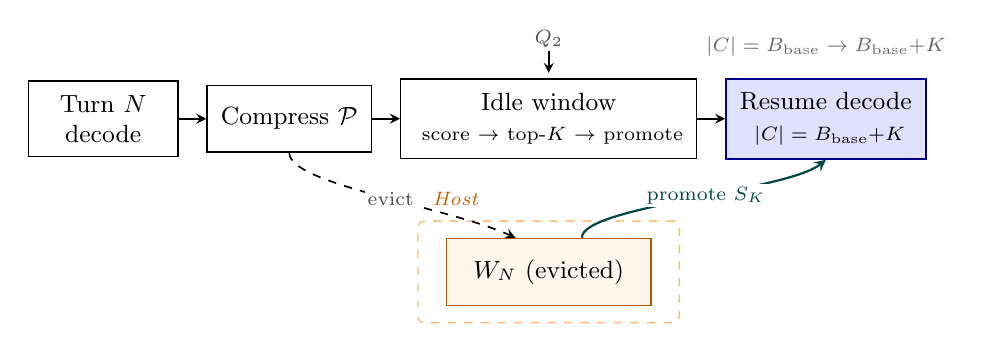
\begin{tikzpicture}[
  >=latex, line width=0.4pt,
  font=\small,
  box/.style={draw=black, fill=white, line width=0.5pt,
              inner sep=5pt, align=center, minimum height=0.85cm},
  active/.style={box, fill=blue!12, draw=blue!55!black, line width=0.7pt},
  store/.style={box, fill=orange!8, draw=orange!70!black},
  arr/.style={->, line width=0.6pt, draw=black, >=stealth},
  promarr/.style={->, line width=0.8pt, draw=teal!55!black, >=stealth},
  arrlabel/.style={font=\scriptsize, text=black!70, fill=white, inner sep=1pt},
  groupbox/.style={draw=orange!55, dashed, line width=0.5pt, rounded corners=2pt},
  grouplabel/.style={font=\scriptsize\itshape, text=orange!75!black},
  bodysmall/.style={font=\scriptsize, text=black!75}
]
  % --- Top tier: horizontal pipeline ---
  \node[box, minimum width=1.9cm] (dN) at (0, 0) {Turn $N$\\decode};
  \node[box, minimum width=1.7cm, right=10pt of dN]   (cmp)  {Compress~$\mathcal{P}$};
  \node[box, minimum width=2.7cm, right=10pt of cmp]  (idle) {Idle window\\
        {\scriptsize{} score~$\to$~top-$K$~$\to$~promote}};
  \node[active, minimum width=2.1cm, right=10pt of idle] (resume)
        {Resume decode\\{\scriptsize{} $|C|=\bbase{+}K$}};

  % --- Sequential arrows, all solid + same style ---
  \draw[arr] (dN) -- (cmp);
  \draw[arr] (cmp) -- (idle);
  \draw[arr] (idle) -- (resume);

  % --- Q_2 input from above ---
  \draw[arr] ([yshift=10pt]idle.north) -- ([yshift=2pt]idle.north);
  \node[arrlabel, anchor=south] at ([yshift=10pt]idle.north) {$Q_2$};

  % --- Bottom tier: single host store ---
  \node[store, minimum width=2.6cm, below=1.0cm of idle] (wn) {$W_N$ (evicted)};

  % Dashed host group and its label
  \node[groupbox, fit=(wn), inner xsep=10pt, inner ysep=6pt] (hgroup) {};
  \node[grouplabel, anchor=south west]
       at ([xshift=2pt, yshift=2pt]hgroup.north west) {Host};

  % --- Evict (down) and promote (up) ---
  \draw[arr, dashed]
       (cmp.south) .. controls ([yshift=-0.4cm]cmp.south)
                              and ([yshift=0.4cm]wn.north west) ..
       ([xshift=-12pt]wn.north)
       node[arrlabel, pos=0.55] {evict};

  \draw[promarr]
       ([xshift=12pt]wn.north) .. controls ([xshift=12pt, yshift=0.4cm]wn.north)
                                          and ([xshift=-0.5cm, yshift=-0.4cm]resume.south) ..
       (resume.south)
       node[arrlabel, text=teal!55!black, pos=0.55] {promote~$S_K$};

  % --- |C| growth indicator: small inline note above resume box ---
  \node[bodysmall, text=black!60, anchor=south]
       at ([yshift=4pt]resume.north) {$|C|=\bbase \to \bbase{+}K$};
\end{tikzpicture}
\end{document}
